\documentclass[thesis.tex]{subfiles}
\begin{document}

\chapter{Methodology}\label{chap:basics}

In this chapter we describe how the provided MRI Volume Data with the masked Aortic Dissections are used in this thesis. In the first step we go along the centerlines of the lumen using a fixed step size to obtain the cross-sections at each position. Then, we extract the contours of the TL and FL from the cross-sections. In the third step we convert the found contours into chain codes. We then apply the fourier transform on the chain codes to obtain EFDs. We then use the EFDs to approximate the lumen shapes and correct overlapping contours that might occur. The result can then be used for visualization, rendering, interpolation etc.. We also add a vessel wall around the result for rendering. An overview of this pipeline is shown in figure \ref{bla}. We demonstrate all methods on a phantom data set thoughout this chapter. 

\section{Obtaining Cross-Sections}
In this step of the pipeline we describe how cross-sections are obtained from the provided volume data.The provided data contains three centerlines, the centerline of the FL, the centerline of the TL , and the TCL. The TCL interpolates points that lie between the centerlines of the TL and FL. All centerlines are modeled by interpolating B-Splines. To obtain cross-sections, we go along the splines using a fixed step size and compute the local coordinate system at each position we visit on the spline. The step size is computed by dividing the length of the spline by the number of cross-section, which is a parameter the user can provide.
By default the cross-sections are obtained from the TCL, but the user can also choose to use the centerlines of the TL and FL instead. \\
The difference of those options is that when we use the TCL, we obtain only one set of cross-sections that can be used for both lumen in all other steps in the pipeline. The set of cross-sections then also contains exactly as many cross-sections as chosen by the user. When using the centerlines of the FL and TL instead, we obtain two different sets of cross-sections and each of the sets contains as many cross-sections as the set of cross-sections obtained by using the TCL. Another difference is that when we use the TCL to obtain cross-section we only have one fixed step size that is used while going along the spline. When we use the centerlines of the FL and TL instead, we have two different fixed step sizes, because the step size depends on the length of the respective centerline.

These differences make it complicated to use the cross-sections obtained from the centerlines of the FL and TL in some steps of the pipeline. For example in the step of the pipeline in which we correct the overlapping of the reconstructed contours we have to identify both lumen in each cross-section. In the case the cross-sections were obtained by using centerlines of the FL and TL, we can either ignore the parameter that controls the number of cross-sections to be used and process all cross-sections, or we have to decide which cross-sections to use.

The centerline of the TL is usually longer than the centerline of the FL. This means we cannot assume that the n-th cross-section of the TL is anywhere near the n-th cross-section of the FL. If we were to use only cross-sections from the FL centerline, we would not cover the whole TL. On the other hand, if we were to use only cross-sections of the TL centerline, the step size could be too large and some important features of the FL could be skipped. By using the TCL as default we avoid those problems. In case the user wants to use the other centerlines instead those steps will be skipped. An example of a cross-section can be seen in figure \ref{fig:cross-section}.

\begin{figure}[h]
\centering
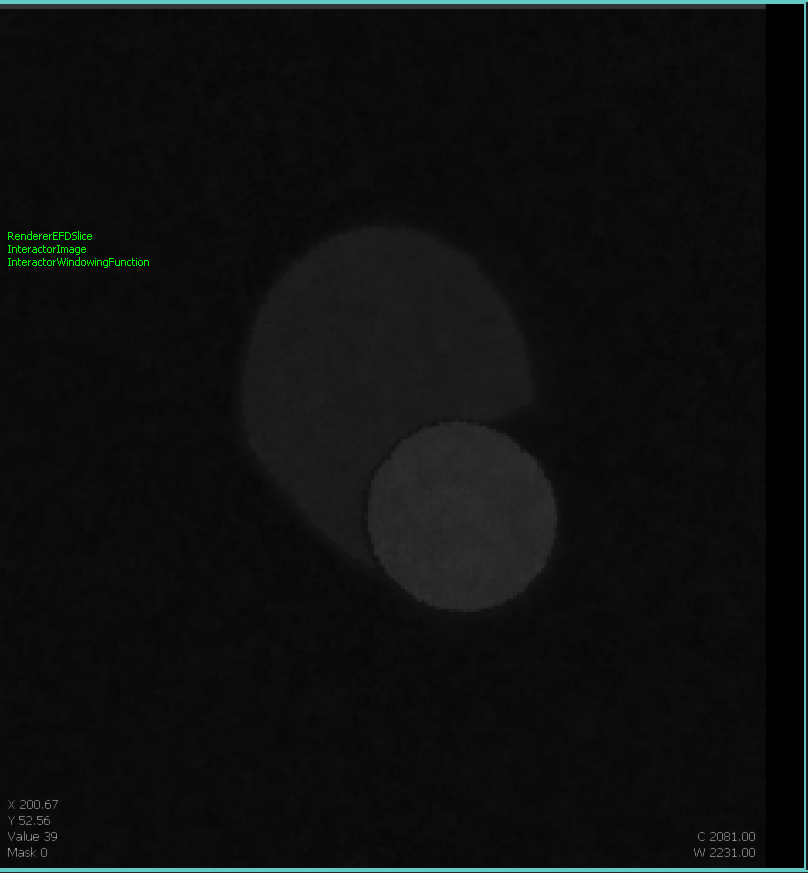
\includegraphics[width=\textwidth/2]{cross-section249.png}
\caption{A cross-section of the phantom data set. In the center both lumen are visible. The TL is the almost perfect circular lumen with brighter intensity values than the FL. The FL is the non-circular lumen that winds arounds the TL.}
\label{fig:cross-section}
\end{figure}  

\begin{figure}[h]
\centering
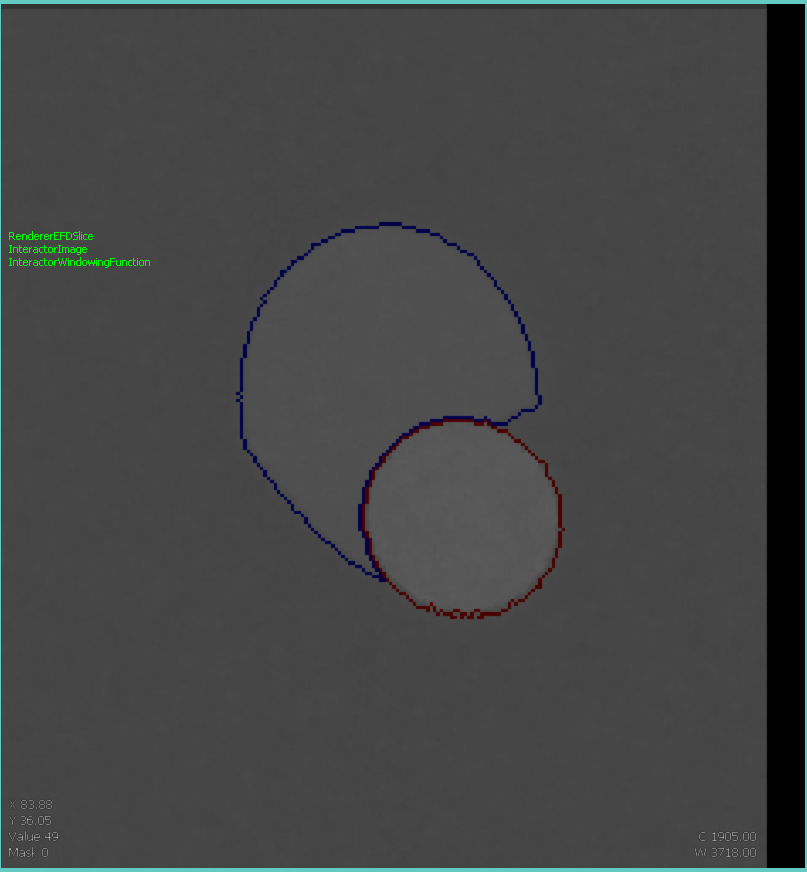
\includegraphics[width=\textwidth/2]{cross-section249_with_extracted_contours.png}
\caption{The same cross-section as in \ref{fig:cross-section} after extracting the lumen contours. In the center both lumen are visible and their respective contours overlayed. The contour of the FL is colored blue, while the contour of the TL is colored red. Compared to \ref{fig:cross-section} the windowing function was adjusted for better visibility of the contours.}
\label{fig:extracted_contours}
\end{figure} 

\section{Extracting Lumen Contours}
Both lumen are masked in our data, so we can identify pixels belonging to the lumen when traversing the cross-sections. In some cases there are several disconnected components for each lumen as shown in figure \ref{bla}.That is why we first iterate over each cross-section to find the largest connected component, which will be used  in all further steps. We use a modified version of the Moore-Neighborhood-Tracing algorithm to follow the contour. The only difference is that we do not backtrack, but instead go right of the current relative direction. The algorithm still has all advantages and disadvantage sof the original Moore-Neighborhood-Tracing algorithm. An example of the extracted contours can be seen in figure \ref{fig:extracted_contours}.

\section{Converting Contour to Chain Code}
After we extracted the contours of the cross-sections we convert them to chain codes. This is mainly done to achieve translation invariance. The Encoding Scheme we use is the Freeman Chain Encoding Scheme that we described in section ... . 

\section{Computing Elliptic Fourier Descriptors}
In this step we have to compute the EFDs that will be used to represent the shapes of the lumen. As the EFDs are a set of fourier coefficients, we have to use the Discrete Fourier Transform on the chain codes we obtained in the last step of the pipeline. More specifically, we use the DFT defined in \cite{giardinia}. The Fourier approximation for the 2D case is then defined as:

\begin{equation} \label{eq:dft_x}
 x(t) = A_0 + \sum_{n=1}^{N} a_n cos \frac{2\pi n t}{T} + b_n sin \frac{2\pi n t}{T}
\end{equation}


\begin{equation} \label{eq:dft_y}
 y(t) = C_0 + \sum_{n=1}^{N} c_n cos \frac{2\pi n t}{T} + d_n sin \frac{2\pi n t}{T}
\end{equation}
 
with $ A_0$ and $C_0 $ being the DC Components. $N$ is the total number of harmonics to be used, which can be freely changed by the user. $a_n$, $b_n$, $c_n$, and $d_n$ are fourier coefficients. $t$ is the elapsed time, and $T$ is the total time needed for one period. \\ In our implementation we use this definition of the Fourier Approximation to reconstruct the contour in a gapless manner, if it is necessary to do so. However, for most steps of our pipeline and for many rendering applications it is sufficient to reconstruct the signal using less reconstruction points. The main advantages of using less reconstruction points is the reduced memory consumption and faster processing due to the lower number of points that need to be processed. For this purpose we also implemented another fourier approximation that is very similar to the one defined in \ref{eq:dft_x} and \ref{eq:dft_y}. The only differences are that we set $t$ to be the index of the current reconstruction point and $T$ to be the total number of reconstruction points that should be used. This changes cause the reconstructed points to be placed equidistantly on the reconstructed contour and allow the user to freely adjust the total number of reconstruction points.\\ 

The DC Components $A_0$ and $C_0$ correspond to the x- and y-coordinate of the centroid of the input signals and are defined as: 

\begin{equation} \label{eq:dft_dc_x}
 A_0 =  \frac{1}{T} \sum_{p=1}^{K} \bigg[ \frac{\Delta x_p}{2 \Delta t_p} (t_p^2 - t_{p-1}^2) + \xi_p(t_p - t_{p-1})\bigg]
\end{equation}  

\begin{equation} \label{eq:dft_dc_y}
 C_0 =  \frac{1}{T} \sum_{p=1}^{K} \bigg[ \frac{\Delta y_p}{2 \Delta t_p} (t_p^2 - t_{p-1}^2) + \delta_p(t_p - t_{p-1})\bigg]
\end{equation}   
with

\begin{equation} \label{eq:dft_xi}
 \xi_p =  \sum_{j=1}^{p-1} \Delta x_j - \frac{\Delta x_p}{\Delta t_p} \sum_{j=1}^{p-1}\Delta t_j
\end{equation}  

\begin{equation} \label{eq:dft_delta}
 \delta_p =  \sum_{j=1}^{p-1} \Delta y_j - \frac{\Delta y_p}{\Delta t_p} \sum_{j=1}^{p-1}\Delta t_j
\end{equation}  
 
\begin{equation} \label{eq:dft_delta_first}
 \delta_1 =  \xi_1 = 0
\end{equation} 
 
We directly compute the 4 fourier coefficients of the $n$-th harmonic using the following equations:

\begin{equation} \label{eq:dft_a_n}
 a_n = \frac{T}{2n^2\pi^2} \sum_{p=1}^{K}\frac{\Delta x_p}{\Delta t_p}[cos\frac{2n\pi t_p}{T} - cos\frac{2n\pi t_{p-1}}{T}]
\end{equation} 

\begin{equation} \label{eq:dft_b_n}
 b_n = \frac{T}{2n^2\pi^2} \sum_{p=1}^{K}\frac{\Delta x_p}{\Delta t_p}[sin\frac{2n\pi t_p}{T} - sin\frac{2n\pi t_{p-1}}{T}]
\end{equation}
 
\begin{equation} \label{eq:dft_c_n}
 c_n = \frac{T}{2n^2\pi^2} \sum_{p=1}^{K}\frac{\Delta y_p}{\Delta t_p}[cos\frac{2n\pi t_p}{T} - cos\frac{2n\pi t_{p-1}}{T}]
\end{equation} 

\begin{equation} \label{eq:dft_d_n}
 d_n = \frac{T}{2n^2\pi^2} \sum_{p=1}^{K}\frac{\Delta y_p}{\Delta t_p}[sin\frac{2n\pi t_p}{T} - sin\frac{2n\pi t_{p-1}}{T}]
\end{equation}

It should be noted that when using chain codes as input signals, $T$ is the euclidic length of the contour and the elapsed time $t_p$ is the euclidic length from the starting pixel up to the current chain code segment. If the Freeman Chain Code is used, the euclidic length of a segment is 1 for chain code segments 0, 2, 4, and 6 and $\sqrt{2}$ for all other chain code segments. $K$ is the number of chain code segments. $\Delta x_p$ and $\Delta y_p$ are the x- and y-displacement of the current chain code segment compared to the last chain code segment. For example the Freeman chain code segments that encode a movement to the right, 0, 1, and 7, have an x-displacement of 1. Chain Code segments that encode a movement to left instead have a x-displacement of -1 and all other chain code segments have an x-displacement of 0. The same principle applies for the y-displacement, but in vertical direction.

\section{Correcting of overlapping contours}
In this step we ensure that the reconstructed contours do not overlap. This can happen if not sufficient harmonics were used during the computation of the EFDs. For this purpose we iterate over the cross-sections and retrieve the EFDs that describe the contours found in the cross-sections. In our implementation the EFDs are stored in a way that allows us to do so. Additionally, we can differentiate to which lumen each EFD belongs. By doing the iteration using the cross-sections we end up with two EFDs in each iteration. The first EFD describes the FL contour in the current cross-section, while the other describes the lumen contour of the TL. 
The algorithm to correct the overlapping contours can be summarized in the following five steps:

\begin{enumerate}
\item Create a layer for each lumen and draw the reconstructed contours into the corresponding layer
\item Fill the area outside of the reconstructed contour
\item For the FL, fill the area inside of the contour
\item Combine the layers in a specific way
\item Search for the corrected contours in the combined layer
\end{enumerate}

We will now describe each of these steps in detail. In the first step we create an empty image for each of the EFDs. We refer to them as \textit{layers}. Each layer has the same size as a cross-section and is initially filled with black pixels. Then we reconstruct the contours for both lumen using the EFDs. The contours are reconstructed in a gapless manner and they are drawn into their corresponding layers. When drawing the reconstructed contours, it is important to ensure that the drawn contours can still be differentiated, for example by choosing different drawing colors / pixel intensities. 

In the second step, we want to fill the area outside of the contours in both layers. The reason for doing this is that we actually want to fill the area inside the FL. By filling the area outside of the contours,  we can trivially determine pixels inside of the contour. At the time of implementation we did not know of another way to do this. A possible different solution that we did not implement would be to use the methode described in \cite{inside_contour}.  To fill the area outside the  contours we determine a pixel outside the contour, that is used as a starting pixel for the area filling. We determine this pixel by iterating over the pixels in each layer until we find a pixel belonging to the reconstructed contour. In our implementation we iterate over the pixels from left to right, top to down. Therefore, when we find a pixel we can ensure that the pixel above the found pixel is a black pixel that lies outside of the contour.The only exception is when the found pixel is on the top border of the layer, but that would mean that the cross-sections might be too small to fit the whole lumen. In that case the size of the cross-sections should be increased until the whole lumen fits inside without being on any border of the cross-section. \\  Starting from the black pixel above the found pixel we then fill the area outside of the contour with a specific color that differens from both colors that were used to draw the reconstructed contours. For the area filling we first add the black pixel to a list. Then we repeat the following: For each pixel on the list we check all pixels in the 4-neighborhood. If a checked pixel does not belong to the reconstructed contour and it's color is not the same as filling color, we add this pixel to the list and set the pixels color to be the filling color. After all pixels in the neighborhood of a pixel are checked, we remove the current pixel from the list. The algorithmn finishes when no more pixels are on the list. \\
After filling the area outside of the contour, we then want to fill the inside of the contour. Since the layers were initialized with black pixels, the inner area of both drawn reconstructed contours is filled with black pixels. That is why we only need to fill the area inside the contour for one of the layers. The color used for filling the inside of the contour is the same as the color that was used to draw the respective contour. We determine a pixel inside the contour by iterating over the pixels of the layer until we find a black pixel and we use this black pixel as a starting pixel to fill the inside area of the contour the same way we did when we filled the area outside of the contour. \\
In the next step we combine both layers. We first create an image with the same size as the layers and initialize it with black pixels. For each pixel of this empty image, we check the pixels in both layers that have the same coordinates as the current pixel in the new image. If the pixel in the TL layer belongs to the reconstructed TL contour or to the inside area of the reconstructed TL contour, we set the color of the current pixel to be the same as in the TL layer. Otherwise, we check if the pixel in the FL layer belongs to the reconstructed FL contour or the area inside of the FL contour. If it does, we set the color of the current pixel to be the same as in the FL layer. If none of these cases applies, we ignore the current pixel.\\
In the last step we extract the contours from the image that contains the combined layers. We do this by using the same method as in the second step of the pipeline. The obtained contours do not overlap, because the pixels in the TL layer were prioritized over the pixels in the FL layer when we combined both layers.        



\subfilebib % Makes bibliography available when compiling as subfile
\end{document}